\makeatletter
\def\BState{\State\hskip-\ALG@thistlm}
\makeatother

\chapter{Automatic syllable and phoneme segmentation}\label{chap:segmentation}
% \begin{epigraphs}
%   \qitem{...the first beat (sam) is highly significant structurally, as it frequently marks the coming together of the rhythmic streams of soloist and accompanist, and the resolution point for rhythmic tension.}{\citeA[p. 81]{clayton:00:time}}
% \end{epigraphs}

Automatic syllable and phoneme segmentation of singing voice is an important \gls{MIR} task. It provides preliminary syllable or phoneme time boundary and label information to achieve a fine-grained singing voice assessment.

Syllable and phoneme segmentation aim to time-align a piece of singing voice audio recording with syllable or phoneme sequence. It tags the recording with the time-aligned syllable or phoneme boundary timestamps and labels. Within the context of jingju music, syllable and phoneme segmentation aim to time-align a recording with a syllable sequence in pinyin format or a phoneme sequence in \gls{X-SAMPA} format.

This chapter aims to address the automatic syllable and phoneme segmentation task within the context of jingju music, presenting several methods and an evaluation of these methods. The main aims of this chapter are:

\begin{enumerate}[leftmargin=*]

\item To address automatic syllable and phoneme segmentation task for jingju music. The problem is formulated in two ways -- duration-informed lyrics-to-audio alignment and duration-informed syllable or phoneme onset detection. Several approaches are proposed to address the problem.
\item To present a detailed description of hidden semi-Markov model-based (\gls{HSMM}) segmentation method and the proposed onset detection-based method for syllable and phoneme segmentation.
\item To present an evaluation of \gls{HSMM}-based alignment method and the proposed onset detection-based method and explore various deep learning architectures to improve the onset detection-based method.
\end{enumerate}

\section{Task description}\label{sec:ch5:description}

We describe the automatic syllable and phoneme segmentation task addressed in this dissertation. We will also describe how the set of approaches described in this chapter can be adapted to this task, making the task of syllable and phoneme segmentation flexible to the available audio recordings and the related annotations. The task description presented in this section is continued building on the problem formulation presented in \secref{sec:ch3:segmentation_formulation}. 

Given the singing audio recording pre-segmented into pieces of melodic line level, and the prior coarse syllable or phoneme duration information extracted from the musical score or the annotation of teacher's recording, the most relevant syllable and phoneme segmentation tasks for jingju music are duration-informed lyrics-to-audio alignment or duration-informed syllable or phoneme onset detection. In the context of jingju music, lyrics-to-audio alignment aims to time-align the a priori phoneme sequence in \gls{X-SAMPA} format with the melodic line singing audio piece. The coarse phoneme duration information can be incorporated into the alignment system by using an \gls{HSMM}-based model, which sets up the baseline segmentation system stemmed from various \gls{HMM}-based text-to-speech alignment and lyrics-to-audio alignment methods presented in \secref{sec:ch2:text_speech_alignment} and \secref{sec:ch2:lyrics_audio_alignment}. Syllable and phoneme onset detection aim to find the onset timestamps for the syllables and phonemes in a melodic line singing audio piece. The a priori syllable and phoneme duration information can be used as a post-processing step in the detection algorithm to help select the correct onsets. In the context of this dissertation, because the a priori duration information is always accompanied with syllable or phoneme label, the post-processing onset selection method using a priori duration information is equal to time-aligning the syllable or phoneme sequence with the melodic line singing audio piece. 

The two main tasks of this chapter are setting up the \gls{HSMM}-based baseline segmentation method and proposing the onset detection-based segmentation method. As the third task of this chapter, we explore various deep learning architectures for the syllable onset detection and try to identify and explain the most efficient architecture. The performance of all the three tasks will be evaluated on \gls{ASPS}\textsubscript{1} and \gls{ASPS}\textsubscript{2} test datasets. The results and the pros and cons of two segmentation methods and various deep learning architectures will be discussed in detail.

\section{Prerequisite processing}

In this section, we present two prerequisite processings that will be used in the segmentation approaches -- logarithmic Mel input representation and a priori coarse duration model. The former converts the singing voice audio waveform to a perceptual representation - Mel spectrogram, which is then used as the input representation of both \gls{HSMM}-based and onset detection-based segmentation methods. The latter utilizes the coarse syllable or phoneme durations extracted from the annotation of teacher's recording to build the duration model, as the teacher's recording and its annotation is always prior information for an assessment system. The phoneme duration model is then integrated into the \gls{HSMM}-based segmentation method as the state occupancy distribution, and the syllable and phoneme duration models are both used in the onset detection-based segmentation method to help select the correct syllable and phoneme onsets.

\subsection{Logarithmic Mel input representation}\label{sec:ch5:input_representation}

We use \textsc{Madmom} \cite{Bock2016} Python package to calculate the log-mel spectrogram of the singing voice audio. The frame size and hop size of the spectrogram are respectively 46.4ms (2048 samples) and 10ms (441 samples). The low and high frequency bounds of the log-mel calculation are 27.5Hz and 16kHz. We use log-mel input features with a overlapped context window of 15 frames and 80 bins as the input to the networks. The classification acoustic model used in \gls{HSMM}-based segmentation task takes a categorical phoneme label for every context window. While the onset detection model takes a binary onset/non-onset decision sequentially for every context window. This audio pre-processing configuration is almost the same as in Schl\"{u}ter and B\"{o}ck's work \cite{Schluter2014} except that 3 input channels with respectively frame sizes 23ms, 46ms and 93ms have been used in their work, whereas only 1 channel with frame size 46.4ms input is used in this research.

\subsection{Coarse duration and \textit{a priori} duration model}\label{sec:pp_coarse_duration}

The syllable durations of the teacher's singing phrase are stored in an array $M^s=\mu^{1} \cdots \mu^{n} \cdots \mu^{N}$, where $\mu^{n}$ is the duration of the nth syllable. The phoneme durations are stored in a nested array $M_p=M^{1}_p \cdots M^{n}_p \cdots M^{N}_p$, where $M^{n}_p$ is the sub-array with respect to the nth syllable and can be further expanded to $M^{n}_p=\mu_{1}^{n} \cdots \mu_{k}^{n} \cdots \mu_{K_{n}}^{n}$, where $K_{n}$ is the number of phonemes contained in the nth syllable. The phoneme durations of the nth syllable sum to its syllable duration: $\mu^{n}=\sum_{k=1}^{K_{n}} \mu_k^{n}$ (figure \ref{fig:coarse_dur}). In both syllable and phoneme duration sequences -- $M^s$, $M_p$, the duration of the silence is not treated separately and is merged with its previous syllable or phoneme.

\begin{figure}[ht!]
    \centering
    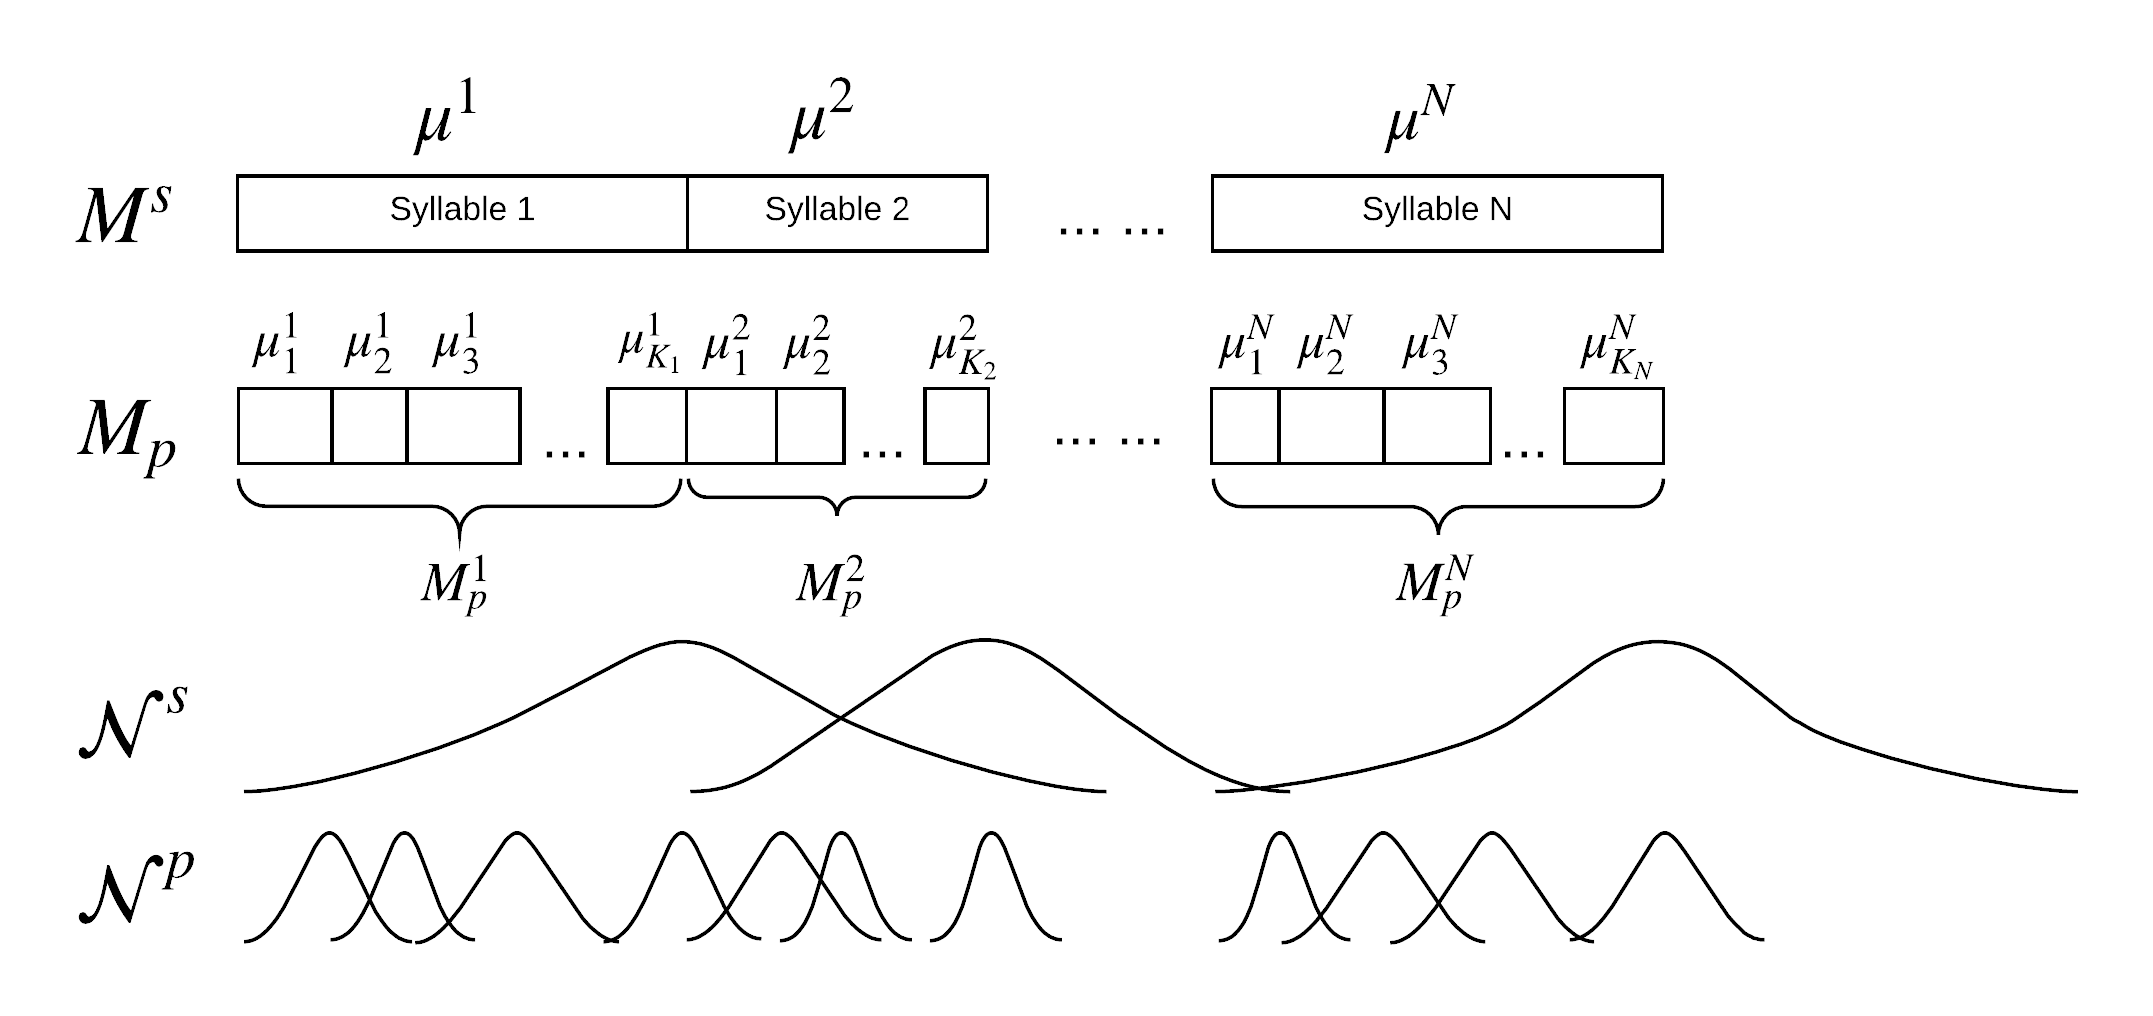
\includegraphics[width=\textwidth]{figs/blockDiags_rong/ch5_coarse_durations_segmentation.png}
    \caption{Illustration of the syllable $M^s$ and phoneme $M_p$ coarse duration sequences and their \textit{a priori} duration models -- $\mathcal{N}^s$, $\mathcal{N}^p$. The blank rectangulars in $M_p$ represent the phonemes.}
    \label{fig:coarse_dur}
\end{figure}

The \textit{a priori} duration model is shaped with a Gaussian function $\mathcal{N} (d; {\mu}_n, \sigma_n^2)$. It provides the prior likelihood of an onset to occur according to the syllable/phoneme duration of the teacher's singing. The mean ${\mu}_n$ of the Gaussian represents the expected duration of nth teacher's syllable/phoneme. Its standard deviation $\sigma_n$ is proportional to $\mu_n$: $\sigma_n=\gamma \mu_n$ and $\gamma$ is heuristically set to 0.35 for the onset detection-based method. Figure \ref{fig:coarse_dur} provides an intuitive example of how the \textit{a priori} duration model works. The a priori phoneme duration model will be used as the state occupancy distribution in the \gls{HSMM}-based segmentation method, and the a priori syllable and phoneme duration models will be incorporated into a duration-informed \gls{HMM} as the state transition probabilities to inform that where syllable/phoneme onsets is likely to occur in student's singing phrase.

\section{HSMM-based segmentation method}\label{sec:ch5:hsmm_segmentation}

As a baseline, we develop an lyrics-to-audio alignment system which also makes use of the prior phoneme duration information. This lyrics-to-audio alignment system is a 1-state monophone \gls{DNN}/\gls{HSMM} model. We use monophone model because our small dataset doesn't have enough phoneme instances for exploring the context-dependent triphones model, also Brognaux and Drugman \cite{brognaux2016hmm} and Pakoci et al. \cite{pakoci2016phonetic} argued that context-dependent model can not bring significant alignment improvement. It is convenient to apply 1-state model because each phoneme can be represented by a semi-Markovian state carrying a state occupancy time distribution. The audio preprocessing step is presented in \secref{sec:ch5:input_representation}.

\subsection{Discriminative acoustic model}

We use a \gls{CNN} with softmax outputs as the discriminative acoustic model. According to the work of Renals et al. \cite{Renals1994Connectionist}, a neural network with softmax outputs trained for framewise phoneme classification outputs the posterior probability $p(q|x)$ ($q$: state, $x$: observation), which can be approximated as the acoustic model at the frame-level if we assume equal phoneme class priors. In Pons et el.'s work \cite{Pons2017Timbre}, a one-layer \gls{CNN} with multi-filter shapes has been designed. It has been experimentally proved that this architecture can successfully learn timbral characteristics and outperformed some deeper \gls{CNN} architectures in the phoneme classification task for a small jingju singing dataset. The convoluational layer of the architecture has 128 filters of sizes $50{\times}1$ and $70{\times}1$, 64 filters of sizes $50{\times}5$ and $70{\times}5$, and 32 filters of sizes $50{\times}10$ and $70{\times}10$. These filters are large in the frequency axis and narrow in temporal axis, which are designed to capture timbral relevant time-frequency spectrogram patterns. A max-pool layer of $2{\times}N'$ follows before the 32-way softmax output layer with 30\% dropout, where $N'$ is the temporal dimension of the feature map. Max-pooling of $2{\times}N'$ was chosen to achieve time-invariant representations
while keeping the frequency resolution. The detailed model architecture is shown in \tabref{table:ch5:cnn_acoustic_model}.

\begin{table}[ht!]
\centering
\caption{One-layer \gls{CNN} architecture of the acoustic model. N' is the temporal dimension of the feature map.}
\label{table:ch5:cnn_acoustic_model}
\begin{tabular}{l}
\toprule
\makecell[l]{Layer1: Conv 128x $50{\times}1$, 64x $50{\times}5$, 32x $50{\times}5$\\128x $70{\times}1$, 64x $70{\times}5$, 32x $70{\times}10$} \\
Layer2: Max-pooling $2{\times}N'$ \\
Layer3: Dropout 0.3\\
Output layer: 29-way softmax\\
\bottomrule
\end{tabular}
\end{table}

\subsubsection{Model training}

We use this one-layer \gls{CNN} acoustic model for the baseline method. The log-mel context window representation presented in \secref{sec:ch5:input_representation} is used as the model input. The target labels of the training set are prepared according to the ground truth annotations. We set the label of a spectrogram context window to its categorical phoneme class. The model predicts the phoneme class posterior probability for each log-mel spectrogram context window.

The model parameters are learned with mini-batch training (batch size 256), adam \cite{kingma2014adam} update rule and early stopping -- if validation loss is not decreasing after 15 epochs. \gls{ELU}s activation functions and weight decay regularization are used in the first convolutional layer.

\subsection{Coarse duration and state occupancy distribution}

The \gls{HSMM}-based segmentation method receives the phoneme durations of teacher's singing phrase as the prior input. The phoneme durations are stored in a collapsed version of the $M^p$ array (section \ref{sec:pp_coarse_duration}): $M_c^p=\mu_{1}^{s1} \mu_{2}^{s1} \cdots \mu_{N_{s1}}^{s1} \cdots \mu_{1}^{sN} \mu_{2}^{sN} \cdots \mu_{N_{sN}}^{sN}$. The silences are treated separately and have their independent durations.

The state occupancy is the time duration of the phoneme state of the student's singing. It is expected in the best case to be the same duration as that of the teacher's singing. However, in the actual scenario, the phoneme duration of the student's singing always deviates from that of the teacher's singing in varying degrees. We build the state occupancy distribution as a Gaussian, which has the same form $\mathcal{N} (d; {\mu_n}, \sigma_n^2)$ as in section \ref{sec:pp_coarse_duration}, where $\mu_n$ indicates in this context the nth phoneme duration of the teacher's singing. We set $\gamma$ empirically to 0.2 as we found this value works well in our preliminary experiment.

We construct an \gls{HSMM} for phoneme segment inference. The topology is a left-to-right semi-Markov chain, where the states represent sequentially the phonemes of the teacher's singing phrase. As we are dealing with the forced alignment, we constraint that the inference can only be started by the leftmost state and terminated to the rightmost state. The self-transition probabilities are set to 0 because the state occupancy depends on the predefined distribution. Other transitions -- from current states to subsequent states are set to 1. We use a one-layer \gls{CNN} with multi-filter shapes as the acoustic model \cite{Pons2017Timbre} and the Gaussian $\mathcal{N} (d; {\mu_n}, \sigma_n^2)$ introduced in section \ref{sec:pp_coarse_duration} as the state occupancy distribution. The inference goal is to find best state sequence, and we use Gu\'{e}don's \gls{HSMM} Viterbi algorithm \cite{GUEDON20072379} for this purpose. The baseline details and code can be found in the Github page\textsuperscript{\ref{ft:github}}. Finally, the segments are labeled by the alignment path, and the phoneme onsets are taken on the state transition time positions.

\subsection{Experimental setup}

We use \gls{ASPS}\textsubscript{1} test dataset presented in \secref{sec:ch4:dataset_segmentation} and two metrics to evaluate the algorithm performance -- onset detection accuracy and percentage of correct segments, where we also consider the phoneme label correctness in calculating onset detection accuracy. These two metrics have been presented in \secref{sec:ch2:evaluation_metrics}. We trained the \gls{CNN} acoustic model 5 times with different random seeds, and report the mean and the standard deviation score on the testing part of the dataset.

\subsection{Results and discussions}\label{sec:ch5:results_hsmm}

We only show the F1-measure of the results of the \gls{HSMM}-based method in \tabref{table:ch5:results_hsmm}. The full results including precision and recall can be found in the Github page\textsuperscript{\ref{ft:github}}. The performance of the \gls{HSMM}-based method is mediocre in the sense that none of the onset detection accuracy and percentage of correct segments reaches an ideal level. The low onset detection accuracy -- 44.5\% for phoneme detection, 41\% for syllable detection, means that the \gls{HSMM}-based method cannot maintain more than half of the detected onsets within the 50ms tolerance window, which is crucial for the onset detection or segmentation of the consonants since they usually have a short duration. The low percentage of correct segments -- 53.4\% for phoneme and 65.8\% for syllable, means that many phoneme boundaries including vowel boundaries are not detected correctly. As a consequence, the segmentation error will propagate to the automatic assessment step and reduce the assessment accuracy. 

\begin{table}[ht]
  \centering
  \caption{Evaluation results table. Table cell: mean score$\pm$standard deviation score.}
  \label{table:ch5:results_hsmm}
  \begin{tabular}{cccc}
    \toprule
        \multicolumn{2}{c}{Onset F1-measure \%} & \multicolumn{2}{c}{Segmentation \%} \\
    phoneme & syllable &  phoneme & syllable \\
    \midrule
    44.5$\pm$0.9 & 41.0$\pm$1.0 & 53.4$\pm$0.9 & 65.8$\pm$0.7 \\
    \bottomrule
  \end{tabular}
\end{table}

\begin{landscape}
\mbox{}\vfill
\begin{figure}[ht!]
    \centering
    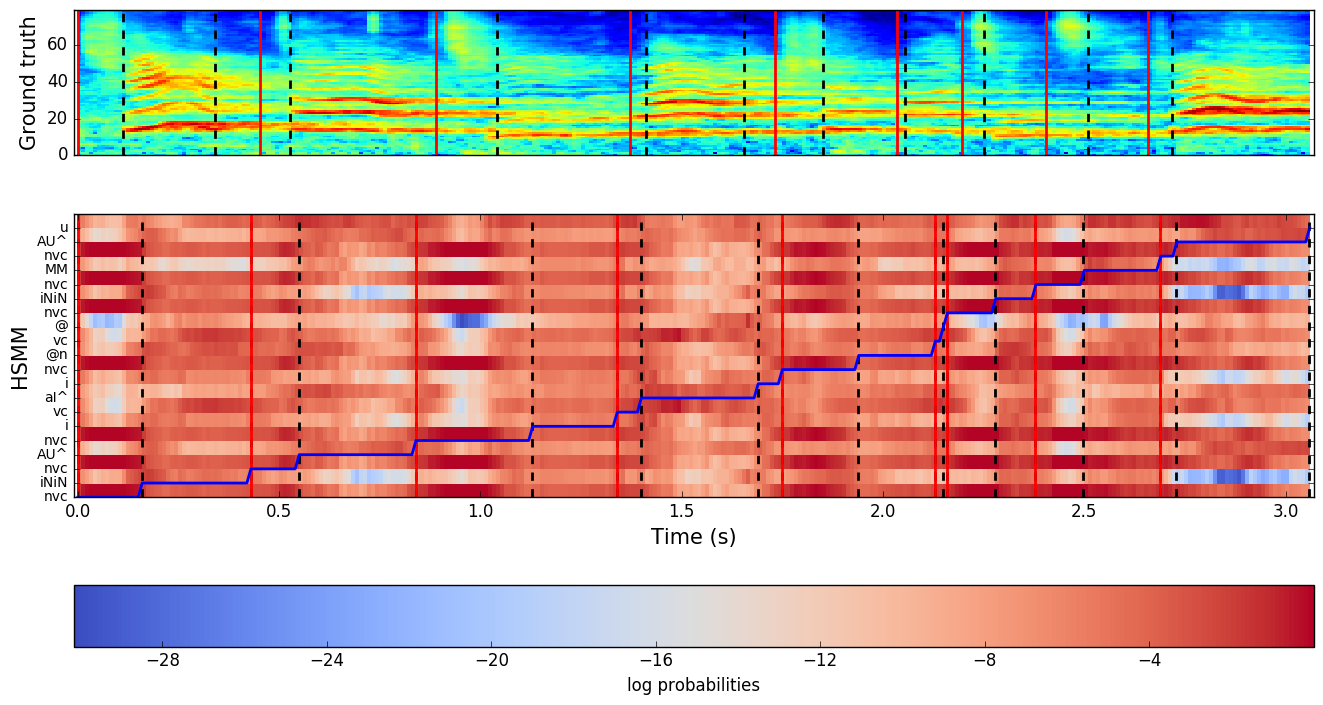
\includegraphics[width=1.4\textwidth]{figs/results/ch5_results_hsmm_baseline.png}
    \caption{An illustration of the result for a singing phrase in the testing part of the dataset. The red solid and black dash vertical lines are respectively the syllable and phoneme onset positions. 1st row: ground truth, 2nd row: HSMM-based segmentation method. The staircase-shaped curve in the 2nd row is the alignment path.}
    \label{fig:ch5:results_example_hsmm}
\end{figure}
\vfill
\end{landscape}

\figref{fig:ch5:results_example_hsmm} shows a result example for a singing phrase in the testing part of the dataset. Notice that there are some extra or missing onsets in the detection. This is due to the inconsistency between the coarse duration input and the ground truth, for example, students might sing extra or miss some phonemes in the actual singing. We can also observe the deviations between the detected and ground truth phoneme onsets. Some of the deviations are quite large, for example, the first detected syllable onset after 2 seconds in the 2nd row, which is an indication that the \gls{HSMM}-based segmentation method cannot meet the need of having a precise segmentation, and it has to be improved or replaced by a better method. 

The unsatisfactory performance of the \gls{HSMM}-based segmentation method might be due to the lack of a large training dataset. The \gls{DNN} acoustic model usually requires a certain amount of training dataset such that it can effectively learn the temporal-spectral patterns of each phoneme class.

\section{Onset detection-based segmentation method}\label{sec:ch5:onset_segmentation}

The unsatisfactory performance of the \gls{HSMM}-based segmentation method motivates us to search for a more accurate segmentation method. As we mentioned in \secref{sec:ch5:results_hsmm}, the lack of enough training dataset might be the cause of the unsatisfactory performance. In this section, we devise a coarse duration-informed syllable and phoneme segmentation method based on syllable and phoneme onset detection. As the onset detection is generally a binary detection problem -- to classify the spectrogram of each frame into onset or non-onset class, it can greatly reduce the amount of the required training dataset. The coarse syllable and phoneme durations extracted from the annotation of teacher's recording can be used in the algorithm to boost the segmentation performance.

In the proposed onset detection-based segmentation method, the syllable and phoneme \gls{ODF}s are jointly learned by a hard parameter sharing multi-task \gls{CNN} model. The syllable/phoneme boundaries and labels are then inferred by an \gls{HMM} using the \textit{a priori} duration model as the transition probabilities and the \gls{ODF}s as the emission probabilities.

\subsection{CNN onset detection function}\label{sec:ch5:cnn_odf}

We build a \gls{CNN} for classifying each log-mel context and output the syllable and phoneme \gls{ODF}s. We extend the \gls{CNN} architecture presented in Schl\"{u}ter's work \cite{Schluter2014} by using two predicting objectives -- syllable and phoneme (figure \ref{fig:cnn_architecture}). The two objectives share the same parameters, and both are using the sigmoid activation function. Binary cross-entropy is used as the loss function. The loss weighting coefficients for the two objectives are set to equal since no significant effect has been found in the preliminary experiment.

\begin{figure}[ht!]
    \centering
    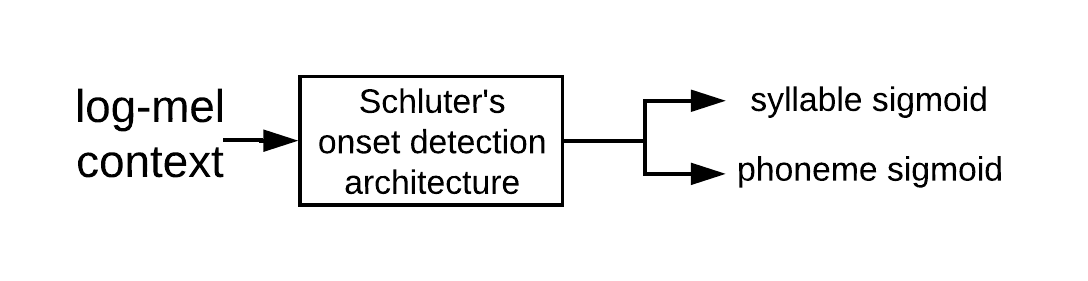
\includegraphics[width=0.8\textwidth]{figs/blockDiags_rong/ch5_cnn_architecture_segmentation.png}
    \caption{Diagram of the multi-task CNN model.}
    \label{fig:cnn_architecture}
\end{figure}

\subsubsection{Model training}

The target labels of the training set are prepared according to the ground truth annotations. We set the label of a certain context to 1 if an onset has been annotated for its corresponding frame, otherwise 0. To compensate the human annotation inaccuracy and to augment the positive sample size, we also set the labels of the two neighbor contexts to 1. However, the importance of the neighbor contexts should not be equal to their center context, thus we compensate this by setting the sample weights of the neighbor contexts to 0.25. A similar sample weighting strategy has been presented in Schluter's paper \cite{Schluter2014}. Finally, for each log-mel context, we have its syllable and phoneme labels. They will be used as the training targets in the \gls{CNN} model to predict the onset presence.

The model parameters are learned with mini-batch training (batch size 256), adam \cite{kingma2014adam} update rule and early stopping -- if validation loss is not decreasing after 15 epochs. The \gls{ODF}s output from the \gls{CNN} model is used as the emission probabilities for the syllable/phoneme boundary inference.

\subsection{Phoneme boundaries and labels inference}\label{sec:ch5:dur_label}

The inference algorithm receives the syllable and phoneme durations and labels of teacher's singing phrase as the prior input and infers the syllable and phoneme boundaries and labels for the student's singing phrase.

We present an \gls{HMM} configuration which makes use of the coarse duration and label input (section \ref{sec:pp_coarse_duration}) and can be applied to inferring firstly (i) the syllable boundaries and labels on the \gls{ODF} for the whole singing phrase, then (ii) the phoneme boundaries and labels on the \gls{ODF} segment constrained by the inferred syllable boundaries. To use the same inference formulation, we unify the notations $N$, $K_n$ (both introduced in section \ref{sec:pp_coarse_duration}) to $N$, and $M^s$, $M^{n}_{p}$ to $M$. The unification of the notations has a practical meaning because we use the same algorithm for both syllable and phoneme inference. The \gls{HMM} is characterized by the following:

\begin{enumerate}[leftmargin=*, itemsep=0pt]
    \item The hidden state space is a set of $T$ candidate onset positions $S_1, S_2, \cdots, S_T$ discretized by the hop size, where $S_{T}$ is the offset position of the last syllable or the last phoneme within a syllable.
    \item The state transition probability at the time instant $t$ associated with state changes is defined by \textit{a priori} duration distribution $\mathcal{N} (d_{ij} ; \mu_t, \sigma_t^2)$, where $d_{ij}$ is the time distance between states $S_i$ and $S_j$ ($j>i$). The length of the inferred state sequence is equal to $N$.
    \item The emission probability for the state $S_j$ is represented by its value in the ODF, which is denoted as $p_j$.
\end{enumerate} 

The goal is to find the best onset state sequence $Q={q_1 q_2 \cdots q_{N-1}}$ for a given duration sequence $M$ and impose the corresponding segment label, where $q_i$ denotes the onset of the $i+1$th inferred syllable/phoneme. The onset of the current segment is assigned as the offset of the previous segment. $q_0$ and $q_N$ are fixed as $S_1$ and $S_T$ as we expect that the onset of the first syllable(or phoneme) is located at the beginning of the singing phrase(or syllable) and the offset of the last syllable(or phoneme) is located at the end of the phrase(or syllable). One can fulfill this assumption by truncating the silences at both ends of the incoming audio. The best onset sequence can be inferred by the logarithmic form of Viterbi algorithm \cite{rabiner1989tutorial}:
% \begin{equation}
% \delta_n(i)= \max_{q_1,q_2,\cdots,q_n}{\log P[q_1 q_2 \cdots q_n,\, \mu_1 \mu_2 \cdots \mu_n]}
% \end{equation}

\begin{algorithm}
\caption{Logarithmic form of Viterbi algorithm using the \textit{a priori} duration model}\label{alg:log_viterbi}
\begin{algorithmic}
\item $\delta_n(i) \gets \max\limits_{q_1,q_2,\cdots,q_n}{\log P[q_1 q_2 \cdots q_n,\, \mu_1 \mu_2 \cdots \mu_n]}$
\Procedure{LogFormViterbi}{$M, p$}

\BState \emph{Initialization}:
\State $\delta_1(i) \gets \log(\mathcal{N} (d_{1i} ; \mu_1, \sigma_1^2))+\log(p_i)$
\State $\psi_1(i) \gets S_1$

\BState \emph{Recursion}:
\State $tmp\_var(i,j) \gets \delta_{n-1} (i) + \log(\mathcal{N} (d_{ij} ; \mu_n, \sigma_n^2))$
\State $\delta_n (j) \gets \max\limits_{1 \leqslant i < j} tmp\_var(i,j) +\log(p_j)$
\State $\psi_n (j) \gets \arg\max\limits_{1 \leqslant i < j} tmp\_var(i,j)$
\BState \emph{Termination}:
% \State $tmp\_var(i) \gets \delta_{N-1} (i) + \log(\mathcal{N} (d_{i T} ; \mu_N, \sigma_N^2))$
% \State $\log P^* \gets \max\limits_{1 \leqslant i < T} tmp\_var(i)$
\State $q_{N} \gets \arg\max\limits_{1 \leqslant i < T} {\delta_{N-1} (i) + \log(\mathcal{N} (d_{i T} ; \mu_N, \sigma_N^2))}$
\EndProcedure
\end{algorithmic}
\end{algorithm}

Finally, the state sequence $Q$ is obtained by the backtracking step. The implementation of the algorithm can be found in the Github link\textsuperscript{\ref{ft:github}}.

\subsection{Experimental setup}

We use \gls{ASPS}\textsubscript{1} test dataset presented in \secref{sec:ch4:dataset_segmentation} and two metrics to evaluate the algorithm performance -- onset detection accuracy and percentage of correct segments, where we also consider the phoneme label correctness in calculating onset detection accuracy. These two metrics have been presented in \secref{sec:ch2:evaluation_metrics}. We trained the onset detection neural network model 5 times with different random seeds, and report the mean and the standard deviation score on the testing part of the dataset.

\subsection{Results and discussions}

We only show the F1-measure of the results of both \gls{HSMM}-based and onset detection-based methods in \tabref{table:ch5:results_onset}. The full results including precision and recall can be found in the Github page\textsuperscript{\ref{ft:github}}. 

\begin{table}[ht]
  \centering
  \caption{Evaluation results of HSMM-based and onset detection-based methods. Table cell: mean score$\pm$standard deviation score.}
  \label{table:ch5:results_onset}
  \begin{tabular}{l|cccc}
    \toprule
    Methods & \multicolumn{2}{c}{Onset F1-measure \%} & \multicolumn{2}{c}{Segmentation \%} \\
            & phoneme & syllable &  phoneme & syllable \\
    \midrule
    HSMM-based & 44.5$\pm$0.9 & 41.0$\pm$1.0 & 53.4$\pm$0.9 & 65.8$\pm$0.7 \\

    \makecell[l]{Onset\\detection-based} & 75.2$\pm$0.6 & 75.8$\pm$0.4 & 60.7$\pm$0.4 & 84.6$\pm$0.3 \\
    \bottomrule
  \end{tabular}
\end{table}

On both metrics -- onset detection and segmentation, the proposed method outperforms the baseline. The proposed method uses the \gls{ODF} which provides the time ``anchors'' for the onset detection. Besides, the \gls{ODF} calculation is a binary classification task. Thus the training data for both positive and negative class is more than abundant. Whereas, the phonetic classification is a harder task because many singing interpretations of different phonemes have the similar temporal-spectral patterns. Our relatively small training dataset might be not sufficient to train a proper discriminative acoustic model with 29 phoneme categories. We believe that these reasons lead to a better onset detection and segmentation performance of the proposed method.

\begin{figure}[ht!]
    \centering
    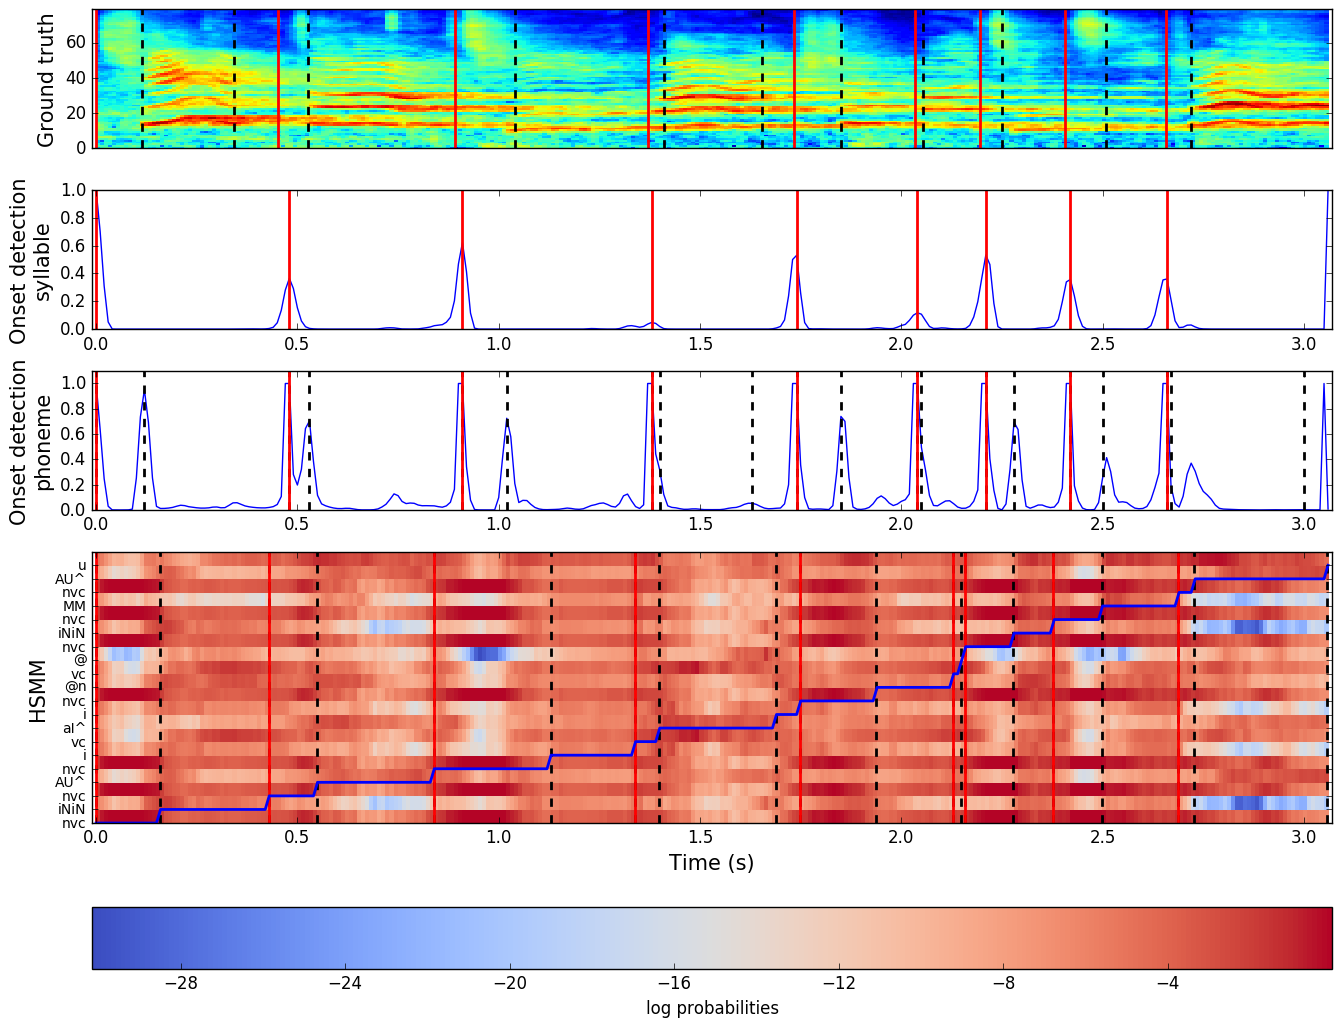
\includegraphics[width=\textwidth]{figs/results/ch5_results_segmentation.png}
    \caption{An illustration of the result for a singing phrase in the testing part of the dataset. The red solid and black dash vertical lines are respectively the syllable and phoneme onset positions. 1st row: ground truth, 2nd and 3rd rows: onset detection-based method, 4th row: \gls{HSMM}-based segmentation method. The blue curves in the 2nd and 3rd row are respectively the syllable and phoneme ODFs. The staircase-shaped curve in the 2nd row is the alignment path.}
    \label{fig:ch5:results_example_onset}
\end{figure}


Fig \ref{fig:ch5:results_example_onset} shows an result example for a singing phrase in the testing part of the dataset. Notice that there are some extra or missing onsets in the detection. This is due to the inconsistency between the coarse duration input and the ground truth, for example, students might sing extra or miss some phonemes in the actual singing. Also notice that in the 3rd row, the two detected phoneme onsets within the last syllable are not in the peak positions of the \gls{ODF}. This is due to that the onsets is inferred by taking into account both \gls{ODF} and the \textit{a priori} duration model, and the latter partially constraints the detected onsets.

The biggest advantage of the proposed method is the language-independency, which means that the pre-trained \gls{CNN} model can be eventually applied to the singing voice of various languages because they could share the similar temporal-spectral patterns of phoneme transitions. Besides, the Viterbi decoding of the proposed method (time complexity $O(TS^2$), $T$: time, $S$: states) is much faster than the \gls{HSMM} counterpart (time complexity $O(TS^2+T^2S)$). To showcase the proposed algorithm, an interactive jupyter notebook demo is provided for running in Google Colab\footnote{\url{https://goo.gl/BzajRy}}. 

\section{Improving the deep learning-based onset detection model}

In the last section, we devised an onset detection-based syllable and phoneme segmentation method which firstly estimates the \gls{ODF} by using a deep learning classification model, then selects the correct onsets on the \gls{ODF} by using a duration-informed \gls{HMM} model. It is obvious that the accuracy of the onset selection step depends on largely on the quality of the \gls{ODF}. Thus, it is necessary to explore an effective and efficient deep learning architecture for estimating the \gls{ODF}.

In this section, we experiment with seven deep learning architectures for estimating syllable onset detection functions to find the most effective and efficient one for the onset detection task. The seven deep learning models are compared and evaluated on a jingju a cappella singing test dataset presented in \secref{sec:ch4:dataset_segmentation}.

\subsection{Deep learning onset detection functions}\label{sec:ch5:nn_onset_improving}

We introduce the neural network setups and training strategies for the experiment which aims to find the most efficient network architecture trained separately on a jingju singing test dataset for syllable onset detection.

\subsubsection{Searching for the most efficient neural network architecture}\label{sec:ch5:architectures_improving}

Following the terminology used in Pons et al.'s work\cite{Pons2017}, we regard a neural network architecture as two parts -- front-end and back-end. According to their work, the front-end is the part of the architecture which processes the input features and maps it into a learned representation. The back-end predicts the output given the learned representation. In this research, we don't restrict the functionality of back-end to prediction. However, we use it as terminology to differentiate from the front-end. We present the front-ends in table \ref{table:frond_ends} and back-ends in table \ref{table:back_ends}. \textbf{\gls{Conv}} means convolutional layer. \textbf{10x} $\boldsymbol{3\times7}$ means 10 filters of which each convolves on 3 frequency bins and 7 temporal frames. All the \gls{Conv} layers use \gls{ReLU} activations. The first \gls{Conv} layer in the front-end B has 6 different filter shapes. Each \gls{Conv} layer in back-end C and D follows by a batch normalization layer to accelerate the training\cite{Ioffe2015}. \textbf{\gls{BiLSTM}s} means bidirectional \gls{RNN} layers with \gls{LSTM} units. In back-end B, both forward and backward layers in \gls{BiLSTM}s have 30 units with Tanh activations. The activation function type of \textbf{Dense} layer -- \gls{ReLU} or Sigmoid used in back-end A depends on the architecture.

\begin{table}[ht!]
\centering
\caption{Architecture front-ends}
\label{table:frond_ends}
\begin{tabular}{c|c}
\toprule
Front-end A & Front-end B \\
\midrule
Conv 10x $3{\times}7$ & \makecell{Conv 24x $1{\times}7$, 12x $3{\times}7$, 6x $5{\times}7$\\24x $1{\times}12$, 12x $3{\times}12$, 6x $5{\times}12$} \\
Max-pooling $3{\times}1$ & Max-pooling $5{\times}1$ \\
Conv 20x $3{\times}3$ & Conv 20x $3{\times}3$ \\
Max-pooling $3{\times}1$ & Max-pooling $3{\times}1$\\
Dropout 0.5 & Dropout 0.5\\
\bottomrule

\end{tabular}
\end{table}

\begin{table}[ht!]
\centering
\caption{Architecture back-ends}
\label{table:back_ends}
\begin{tabular}{c|c}
\toprule
Back-end A  & Back-end B    \\
\midrule
Dense 256 units & Flatten \\
Flatten & BiLSTMs 30 units \\
Dropout 0.5 & Dropout 0.5\\
% \bottomrule     

\toprule
Back-end C  & Back-end D    \\
\midrule
Conv 40x $3{\times}3$ & Conv 60x $3{\times}3$ \\
Conv 40x $3{\times}3$ & Conv 60x $3{\times}3$ \\
Conv 40x $3{\times}3$ & Conv 60x $3{\times}3$ \\
Conv 80x $3{\times}3$ & Flatten \\
Conv 80x $3{\times}3$ & Dropout 0.5 \\
Conv 80x $3{\times}3$ & \\
Conv 135x $3{\times}3$ & \\
Flatten & \\
Dropout 0.5 & \\
\bottomrule
\end{tabular}
\end{table}

We present seven architectures which are the combination pipelines of the front-ends and back-ends. All back-ends are connected with a sigmoid unit to output the \gls{ODF} for the input log-mel contexts.

\noindent\textbf{Baseline}: Front-end A + back-end A with sigmoid activations. This architecture is the same as the one described in Schl\"{u}ter and B\"{o}ck's work \cite{Schluter2014}.

\noindent\textbf{ReLU dense}: Front-end A + back-end A with \gls{ReLU} activations. In Schl\"{u}ter and B\"{o}ck's work \cite{Schluter2014}, using \gls{ReLU} activations in the back-end A caused a drop in performance when evaluating on B\"{o}ck dataset. However, \gls{ReLU} activation function has been shown to enable better training of deeper networks because it has several advantages compared with Sigmoid, such as reducing the likelihood of vanishing gradient \cite{Glorot2011}. We want to (re-)test the performance of \gls{ReLU} activation on both B\"{o}ck and jingju dataset.

\noindent\textbf{No dense}: Front-end A + Flatten layer. We use this architecture to test the effect of removing the dense layer in the baseline.

\noindent\textbf{Temporal}: Front-end B + back-end A with sigmoid activations. This one is similar to the ``Temporal architecture'' presented in Pons et al.'s work \cite{Pons2017}, and uses various filter shapes in the first convolutional layer. In this work, we use 6 different filter shapes which are wide in temporal axis and narrow in frequency axis. Such kind of filter shape design aims to capture the onset spectral-temporal patterns on the spectrogram. It has been shown experimentally that on a smaller jingju dataset, this architecture outperformed the baseline by effectively learning the temporal onset patterns.

\noindent\textbf{BiLSTMs}: Front-end A with time-distributed \gls{Conv} layers + back-end B. This one is similar to the \gls{CRNN}s architectures presented in Vogl et al.'s work \cite{Vogl2017DrumTV}. We use the sequence of the log-mel contexts as the architecture input and we experiment 3 different sequence lengths -- 100, 200 and 400 frames. At the training phase, two consecutive input sequences are overlapped but their starting points are distanced by 10 frames. At the testing phase, the consecutive input sequences are not overlapped. We use this architecture to test the effect of replacing the dense layer in the baseline by \gls{RNN} layer.

\noindent\textbf{9-layers \gls{CNN}}: Front-end A + back-end C. We use this architecture to test the performance of deep \gls{CNN} without using dense layer.

\noindent\textbf{5-layers \gls{CNN}}: Front-end A + back-end D. As our datasets are relatively small, the above 9-layers \gls{CNN} could be overfitting. Thus, we test also this shallow architecture with 5 \gls{CNN} layers.

\begin{table}[ht!]
\centering
\caption{Total numbers of trainable parameters (TNoTP) of each architecture.}
\label{table:parameters}
\resizebox{\columnwidth}{!}{
\begin{tabular}{cccc}
\toprule
Baseline   & ReLU dense   & No dense     & Temporal \\
\midrule
289,273    & 289,273      & 3,161        & 283,687  \\
\toprule
BiLSTMs & 9-layers \gls{CNN} & 5-layers \gls{CNN} &          \\
\midrule
278,341    & 288,286      & 81,541       &      \\
\bottomrule
\end{tabular}
}
\end{table}

The Total numbers of trainable parameters (TNoTP) of each architecture is shown in table \ref{table:parameters}. To keep a fair comparison, we maintain a similar TNoTP between the baseline, \gls{ReLU} dense, Temporal, \gls{BiLSTM}s and 9-layers \gls{CNN} architectures. We reduce the parameter numbers in No dense and 5-layers \gls{CNN} architectures to explore the model efficiency. Notice that 9-layers and 5-layers \gls{CNN}s are not fully-convolutional architectures \cite{Long2015} since we don't perform average pooling to the last \gls{Conv} layer.

\subsubsection{Model training}\label{sec:ch5:model_training_improving}

We use the same target label preparing strategy been described in Schl\"{u}ter and b\"{o}ck's work \cite{Schluter2014}. The target labels of the training set are prepared according to the ground truth annotations. We set the label of a certain context to 1 if an onset has been annotated for its corresponding frame, otherwise 0. To compensate the human annotation inaccuracy and to augment the positive sample size, we also set the labels of the two neighbor contexts to 1. However, the importance of the neighbor contexts should not be equal to their center context. Thus the sample weights of the neighbor contexts are compensated by being set to 0.25. The labels are used as the training targets in the deep learning models to predict the onset presence.

Binary cross-entropy is used as the loss function. The model parameters are learned with mini-batch training (batch size 256), Adam \cite{kingma2014adam} update rule. 10\% training data is separated in a stratified way for early stopping -- if validation loss is not decreasing after 15 epochs. In all experiments, we use \texttt{Keras}\footnote{\url{https://github.com/keras-team/keras}} with \texttt{Tensorflow}\footnote{\url{https://github.com/tensorflow/tensorflow}} backend to train the models.

\subsection{Onset selection}\label{sec:ch5:onset_selection_improving}
The \gls{ODF} output from the model is smoothed by convoluting with a 5 frames Hamming window. Onsets are then selected on the smoothed \gls{ODF}. Two onset selection methods are evaluated.  The first is a peak picking method which has been used in many \gls{MOD} works \cite{Bock2012c, Schluter2014,Vogl2017DrumTV}. We use the \texttt{OnsetPeakPickingProcessor} module implemented in \textsc{Madmom} \cite{Bock2016} package. Please refer to our code for its detailed parameter setting. Another onset selection method is based on the score-informed \gls{HMM} presented in \secref{sec:ch5:dur_label}, which has been used to take advantage of the prior syllable duration information of the musical score.

\subsection{Experimental setup}\label{sec:ch5:eval_improving} 

We use \gls{ASPS}\textsubscript{2} test dataset presented in \secref{sec:ch4:dataset_segmentation} and the metric -- onset detection accuracy presented in \secref{sec:ch2:evaluation_metrics} to evaluate the performance of each algorithms. We report the evaluation results for both peak-picking and score-informed \gls{HMM} onset selection methods on jingju dataset. The pick-peaking results are reported by grid searching the best threshold on the test set, and the score-informed \gls{HMM} results are evaluated directly on the test set since no optimization is needed.

We report only F1-measure in this paper. 
%Other metrics -- precision and recall can be consulted on the Github page\footnote{\url{https://github.com/musicalOnset-ismir2018/musicalOnset-ismir2018}\label{fn:github}}. 
For jingju dataset, to average out the network random initialization effect, each model is trained 5 times with different random seeds, then the average and standard deviation results are reported. To measure the statistical significance of the performance improvement or deterioration, we calculate the Welch's t-test on the 5 training times results for jingju dataset. We report two tails p-value and reject the null hypothesis if the p-value is smaller than 0.05.

\subsection{Results and discussions}

In this section, we report and analyze the results for the most efficient architecture searching experiments. In tables \ref{table:peak_picking_jingju_archi}, the p-value is calculated by comparing each model results with \textbf{Baseline}.

\begin{table}[ht!]
\centering
\caption{Jingju dataset peak-picking (upper) and score-informed HMM (bottom) results of different architectures.}
\label{table:peak_picking_jingju_archi}
\begin{tabular}{l|cc}
\toprule
               & F1-measure & p-value \\
\midrule
Baseline     &76.17$\pm$0.77     & -- \\
ReLU dense     &76.04$\pm$1.02       & 0.840              \\
No dense       &73.88$\pm$0.44       & 0.002              \\
Temporal       &76.01$\pm$0.61       & 0.749              \\
BiLSTMs 100 &78.24$\pm$0.83       & 0.006              \\
BiLSTMs 200 &77.82$\pm$0.68       & 0.013              \\
BiLSTMs 400 &76.93$\pm$0.68       & 0.178              \\
9-layers \gls{CNN}   &73.83$\pm$0.92        & 0.005              \\
5-layers \gls{CNN}   &76.68$\pm$1.04         & 0.457             \\
% \bottomrule
% \end{tabular}
% \end{table}

% \begin{table}[ht!]
% \centering
% \caption{Jingju dataset score-informed HMM results.}
% \label{table:score_informed_jingju_archi}
% \begin{tabular}{l|cc}
\toprule
               & F1-measure & p-value \\
\midrule
Baseline     & 83.23$\pm$0.57     & --        \\  
ReLU dense     & 82.49$\pm$0.28        & 0.057              \\
No dense       & 82.19$\pm$0.44         & 0.021              \\
Temporal       & 83.23$\pm$0.57         & 1                  \\
BiLSTMs 100 & 82.99$\pm$0.31         & 0.479              \\
BiLSTMs 200 & 83.29$\pm$0.37         & 0.882              \\
BiLSTMs 400 & 82.47$\pm$0.54        & 0.087              \\
9-layers \gls{CNN}   & 80.90$\pm$0.67         & 0.001              \\
5-layers \gls{CNN}   & 83.01$\pm$0.76        & 0.649             \\
\bottomrule
\end{tabular}
\end{table}

Observing table \ref{table:peak_picking_jingju_archi} -- the results of jingju dataset, \textbf{\gls{BiLSTM}s 100} and \textbf{200} outperform \textbf{Baseline} with peak-picking onset selection method but not with score-informed \gls{HMM} method. \textbf{9-layers \gls{CNN}} overfits and significantly performs worse than \textbf{Baseline}, which means this architecture is too ``deep" and overfitted for this test dataset (check the Github page\footnote{\url{https://github.com/ronggong/musical-onset-efficient}\label{fn:github}} for its loss curve). \textbf{Temporal} architecture has the p-value of 1 when evaluating by score-informed \gls{HMM} method, and we confirm that it is a coincidence after having checked its 5 training times F1-measures. \textbf{No dense} architecture performs significantly worse than \textbf{Baseline}. However, considering its tiny TNoTP -- 3,161, this performance is quite acceptable. The similar case has been reported in Lacoste and Eck's work\cite{Lacoste2007a}, where their 1 unit 1 hidden layer architecture achieved a remarkable result (only 4\% F1-measure worse than their best architecture). This means that if the state-of-the-art performance is not required, one can use a quite small and efficient architecture. The score-informed \gls{HMM} onset selection method outperform the peak-picking by a large margin. Also notice that the score-informed \gls{HMM} method is able to compensate both good and bad performance of peak-picking, which can be seen by comparing upper and bottom results regarding \textbf{No dense}, \textbf{\gls{BiLSTM}s 100} and \textbf{200} models.

Finally, we choose \textbf{5-layers \gls{CNN}} as the most efficient architecture because it performs consistently equivalent to \textbf{Baseline} but only contains 28.3\% TNoTP. Although \textbf{Temporal} architecture performs equally well, it is not selected because its equal TNoTP to \textbf{Baseline} and the complex configuration of its front-end B. \textbf{\gls{BiLSTM}s} outperforms \textbf{Baseline} on jingju dataset, however, due to its overfitting on B\"{o}ck dataset and slow training, we don't consider it as an efficient architecture.

Experiment code
%full results (precision, recall and F1-measure) 
and pre-trained models used in the experiments are available in Github\footnotemark[\getrefnumber{fn:github}]. A Jupyter notebook running in Google Colab is prepared for showcasing the performance of different network architectures\footnote{\url{https://goo.gl/Y5KAFC}}. 

\section{Conclusions}

We formulate the syllable and phoneme segmentation problem within the context of jingju singing from two different perspectives -- lyrics-to-audio alignment and onset detection. After setting up the baseline \gls{HSMM}-based segmentation (alignment) method, we proposed the duration-informed onset detection-based method for tackling the segmentation problem. Finally, we explored various deep learning architectures for improving the syllable onset detection performance.

A detailed evaluation of \gls{HSMM}-based segmentation method, onset detection-based method and various deep learning onset detection models was discussed for two jingju a cappella singing test datasets. Jingju singing, with distinct musical characteristics, is an ideal case to study the performance of novel methods for syllable and phoneme segmentation.

The duration-informed onset detection-based method explicitly considered coarse syllable and phoneme duration information for the segmentation. However, the algorithm is language-independent, and thus can easily adapt to the singing voice of various languages and even to instrumental playing. Since onset detection-based method is a binary onset/non-onset classification model, it requires a small amount of syllable or phoneme onset annotated training data.

The duration-informed onset detection-based method shows significant promise in syllable and phoneme segmentation task. It provides a significant improvement in both onset detection and segmentation performance compared with the baseline \gls{HSMM}-based method for jingju a cappella singing. An exploration of various deep learning syllable onset detection models showed that the architecture of the deep learning model cannot affect significantly the onset detection performance, however, one can design an efficient architecture to reach the state of the art performance.

One main limitation of the onset detection-based method presented was the assumption that a similar duration of each syllable or phoneme and the same syllable or phoneme sequence should be sung in both teacher's and student's singing pieces. While this is a fair and realistic assumption for jingju professional training since the students can usually imitate the teacher's singing very well, amateur singers might imitate very badly because of a large deviation of the syllable or phoneme duration and missing or extra syllable or phoneme. A coarse syllable and phoneme duration correction might be necessary there before applying the segmentation algorithm. The syllable or phoneme recognition might be the method used to tackle the problem of missing or extra syllable in student's singing.

The onset detection-based segmentation method utilized duration-informed \gls{HMM} to select the correct onsets on the \gls{ODF}. A good quality \gls{ODF} is essential to reach a desirable syllable or phoneme onset detection/segmentation accuracy. Various deep learning architectures were experimented to search for a most effective and efficient one which can lead to a superior syllable onset detection performance. Although the experiment did not show an improvement in onset detection accuracy, we witnessed that a \gls{CNN} architecture without dense connection reached the state of the art performance, while it has much less trainable parameters than the baseline architecture, which indicates that the segmentation model efficiency can be improved by using this deep learning architecture.

The presented onset detection-based segmentation method can be further improved to incorporate other linguistic information such as the phoneme class of each time frame. This is in addition to the ideas explored already -- \gls{HSMM}-based method utilized phoneme class and duration information, while onset detection-based method utilized syllable/phoneme onset and duration information. Such a model which makes use of all of the three information -- onset, phoneme class and duration need to be further explored.

The automatic syllable and phoneme segmentation methods discussed in the chapter are aligned with the goal to lead towards an automatic pronunciation assessment system in a fine granularity for jingju a cappella singing. Syllable and phoneme segmentation is the first step towards this goal. The methods of mispronunciation detection and pronunciation similarity measures are built based on the results of the segmentation.
